\documentclass[UTF8,a4paper,11pt,fontset=fandol,scheme=plain]{ctexart}
\usepackage[margin=23mm,headheight=14pt]{geometry}
\usepackage{amsmath,amssymb,bm,graphicx,booktabs,tabularx,array,caption,float,placeins}
\usepackage{xcolor,enumitem,fancyhdr}
\usepackage[unicode,colorlinks=true,linkcolor=black,citecolor=black,urlcolor=blue!45!black]{hyperref}
\setmainfont{texgyretermes-regular.otf}[BoldFont=texgyretermes-bold.otf,ItalicFont=texgyretermes-italic.otf,BoldItalicFont=texgyretermes-bolditalic.otf]
\setlength{\parindent}{0pt}
\setlength{\parskip}{5pt}
\linespread{1.18}
\setlength{\emergencystretch}{2em}
\setlength{\textfloatsep}{10pt}
\raggedbottom
\renewcommand{\topfraction}{0.95}
\renewcommand{\bottomfraction}{0.85}
\renewcommand{\textfraction}{0.05}
\renewcommand{\floatpagefraction}{0.8}
\setcounter{topnumber}{3}
\setcounter{bottomnumber}{2}
\setcounter{totalnumber}{5}
\makeatletter\setlength{\@fptop}{0pt}\makeatother
\setlength{\intextsep}{12pt}
\renewcommand{\figurename}{图}
\renewcommand{\tablename}{表}
\renewcommand{\refname}{参考文献}
\captionsetup{font=small,labelsep=quad,justification=justified,singlelinecheck=false}
\captionsetup[table]{position=top,skip=6pt}
\ctexset{section={format=\Large\heiti,beforeskip=18pt,afterskip=8pt},subsection={format=\large\heiti,beforeskip=13pt,afterskip=6pt},subsubsection={format=\normalsize\heiti,beforeskip=10pt,afterskip=5pt}}
\pagestyle{fancy}\fancyhf{}\fancyhead[L]{\small 六通道品模与耦合对象库构建 · 近期工作报告}\fancyfoot[C]{\thepage}
\renewcommand{\headrulewidth}{0.3pt}
\newcolumntype{Y}{>{\raggedright\arraybackslash}X}
\setlist{itemsep=2pt,topsep=3pt,parsep=0pt}
\newcommand{\code}[1]{\texttt{\small #1}}
\begin{document}
{\centering\LARGE\heiti 六通道品模与耦合对象库构建\par}
\vspace{4pt}
{\centering\large\heiti ——从滚转通道走向六自由度\par}
\vspace{6pt}
{\centering\small 近期工作报告 · 工作区间：2026-10-26 至 2026-10-31\par}
\vspace{8pt}
\begin{abstract}\noindent \textbf{摘要　}滚转通道验证了“品质相关对象族 → 特权强化学习教师 → 多轮蒸馏统一飞控控制器”的构建路线。将这条路线推广到六自由度，需要一套各通道品质等级同时成立、并且能够对应真实飞机的多通道对象。近期工作按品模构建思维导图实现了从低阶等效传递函数到动力学、再到运动学的六通道品模。依据稳定轴小扰动方程、NASA CR-2144 的 10 架飞机 94 个飞行状态以及 MIL-STD-1797A 与 GJB 2874—1997，设计了交叉通道、长周期、完整惯性耦合与 Dryden 湍流，并经三轮采样形成 v4 六通道对象库。分析表明，保持原滚转通道时横航向只剩两个自由导数；补齐交叉轴判据后，原滚转 1 级对象中仅 9\% 仍为 1 级。据此，对象库改为“模态按 GJB 等级采样、耦合形状取自真实飞机、导数由四次方程精确解出”的构造。v4 库 1/2/3 级各 1,500 个、分布外 500 个，65,536 个候选中 75.6\% 落在真实飞机导数范围内；推导得到的 \(\omega_\phi/\omega_d\) 的 5–95 百分位为 0.73–1.10，与真实飞机的 0.64–1.13 一致；45 项测试全部通过。同期修复了 PPO 实现中采样与更新概率不一致、末步重置后估值两处问题，为后续三回路教师训练准备了修复后的训练源码。\end{abstract}
\noindent \textbf{关键词}　飞行品质；低阶等效系统；六自由度；横航向耦合；对象库；PPO
\vspace{10pt}

\section{工作概述}
\label{sec:overview}
滚转通道研究以 GJB 2874—1997 的滚转模态参数构造了 5,000 个对象，在其上完成了教师训练、多教师蒸馏与跨对象验证。按照品模构建思维导图的“六自由度飞机”分支，下一阶段把对象族扩展到俯仰、滚转与脚蹬三条控制回路。扩展的核心问题有三个：各通道的低阶等效系统如何落到同一套动力学上；交叉通道与长周期等滚转库未覆盖的特性如何设计；以及扩展后的对象是否仍满足各自的品质等级，并能对应真实飞机。

表~\ref{tab:timeline} 列出本阶段的工作及其产物目录。PPO 修复面向后续训练；六通道部分依次经历了解耦实现（v1）、耦合与真实性分析（v2）、重新采样（v3）、合理性检查后的修正（v4）四个版本。各版本对象库独立保存，后一版不覆盖前一版。本阶段聚焦模型、对象库与训练实现，没有开展新的控制器训练，也没有占用 GPU。

\begin{table}[H]
\centering\small
\caption{近期工作与产物（\code{library/} 与 \code{web/} 均位于 \code{six\_channel\_model\_2026-10-29/} 下）}\label{tab:timeline}
\begin{tabularx}{\linewidth}{@{}l>{\raggedright\arraybackslash}p{0.33\linewidth}Y@{}}
\toprule
日期 & 工作 & 产物（仓库内路径） \\
\midrule
10-26 & PPO 概率与末端估值修复 & \code{ppo\_fixes\_2026-10-26/} \\
10-29 & 六通道品模 v1 与联合对象库 & \code{six\_channel\_model\_2026-10-29/pinmo6/}，\code{library/joint\_six\_channel\_5000\_v1/} \\
10-30 & 交叉通道、长周期、惯性耦合与湍流（v2） & \code{library/coupled\_six\_channel\_5000\_v2/}，\code{literature/} \\
10-30 & 品质优先的重新采样（v3） & \code{library/six\_channel\_5000\_v3/} \\
10-31 & 对象库可视化与公式页 & \code{web/} \\
10-31 & 合理性检查与 v4 对象库 & \code{library/six\_channel\_5000\_v4/} \\
\bottomrule
\end{tabularx}
\end{table}

\section{PPO 训练实现的修复}
\label{sec:ppo}
对原交付包所附 PPO 实现的核查发现两处边界问题，分别使概率比和优势估计产生偏差。修复代码以当前 \code{FQControl\_Model/src} 为基准复制到独立目录 \code{ppo\_fixes\_2026-10-26/src}，原交付包、发布仓库源码、冻结实验与权重均保持原样。

\textbf{采样与更新的概率对应同一个值。}Actor 输出高斯采样值 \(\tilde a\)，执行时经限幅得到有界动作 \(a=\operatorname{sat}(\tilde a)\)。原实现在采样时保存 \(\tilde a\) 的对数概率，更新时却对限幅后的 \(a\) 重新求概率，动作饱和时两者不一致，概率比随之偏离。修复后 Actor 新增 \code{sample\_for\_ppo()}，同时返回 \(a\) 与 \(\tilde a\)；缓存保存 \(\tilde a\)，概率比在同一个值上计算：
\begin{equation}
r_t(\vartheta)=\frac{\pi_\vartheta(\tilde a_t\mid s_t)}{\pi_{\vartheta_{\mathrm{old}}}(\tilde a_t\mid s_t)},\qquad a_t=\operatorname{sat}(\tilde a_t).
\end{equation}
原 \code{act()} 的三个返回值及确定性推理接口保持兼容。

\textbf{末端价值取自真实末态。}每个回合按 8 秒截断。原环境在末步自动重置，训练器随后从重置后的初始状态取价值作自举。修复后训练采样使用 \code{env.step(..., auto\_reset=False)}，按连续控制任务的时间截断处理，在重置前计算末端价值，下一轮采样开始时再显式重置：
\begin{equation}
\delta_T=r_T+\gamma\,V\bigl(s_{T+1}^{\mathrm{final}}\bigr)-V(s_T).
\end{equation}
其他环境调用仍默认自动重置。网络结构、权重键、动作限幅、奖励、对象生成、训练配置默认值与优化预算不变。日志、检查点与汇总中新增协议标记 \code{ppo-raw-sample-final-state-v2}，用于区分修复后的实现。另为 NumPy 1.26 的 \code{np.trapz} 与 2.x 的 \code{np.trapezoid} 补充了等价兼容。

8 项 CPU 回归测试全部通过，覆盖双向饱和时的概率比与梯度、旧权重与确定性接口、末态保留、自动与逐行重置、GAE 以及训练器数据流；集成测试中的优化器 step 替换为空操作。后续新增 PPO 训练使用这份修复源码并写入新的结果目录。历史教师按原实现训练，其受影响范围需要对照实际训练版本与日志确定。

\section{六通道品模}
\label{sec:v1}
\subsection{从传递函数到动力学与运动学}
GJB 2874—1997 用低阶等效系统（LOES）描述各通道对驾驶员操纵力的响应，并把品质要求写在等效参数上。品模链路如下：输入为俯仰杆力 \(F_s\)、横向杆力 \(F_{as}\) 与脚蹬力 \(F_{rp}\)（单位 N，拉杆、右压杆、右蹬为正）；按飞行品质采样的 LOES 给出动力学输出 \(V,\alpha,q,\beta,p,r\)（另给出 \(n_z\)、\(\gamma\)）；运动学把稳定轴角速度转到机体轴，用旋转矩阵传播姿态并积分位置，得到思维导图规定的状态
\begin{equation}
\mathbf x=[\,V,\ \alpha,\ q,\ \theta,\ \beta,\ p,\ r,\ \phi,\ \psi,\ X,\ Y,\ Z\,]^{\mathsf T}.
\end{equation}
表~\ref{tab:channels} 给出六个通道的实现形式。

\begin{table}[H]
\centering\small
\caption{六个通道的低阶等效形式（v1）}\label{tab:channels}
\begin{tabularx}{\linewidth}{@{}l>{\centering\arraybackslash}p{0.47\linewidth}Y@{}}
\toprule
通道 & 形式 & 来源 \\
\midrule
\(q\) & \(\dfrac{q}{F_s}=\dfrac{K_\theta(s+1/T_{\theta2})e^{-\tau_\theta s}}{s^2+2\zeta_{sp}\omega_{sp}s+\omega_{sp}^2}\) & GJB A5.1.1.1；扫描页写作 \(\dot\theta/F_s\)，正文为俯仰速率 \\[8pt]
\(\alpha\) & \(\dfrac{\alpha}{F_s}=\dfrac{K_\theta e^{-\tau_\theta s}}{s^2+2\zeta_{sp}\omega_{sp}s+\omega_{sp}^2}\) & 思维导图：\(\gamma/\theta=1/(T_{\theta2}s+1)\)，\(\alpha=\theta-\gamma\) \\[8pt]
\(n_z\) & \(\dfrac{n_z}{F_s}=\dfrac{K_\theta\,(n/\alpha)\,e^{-\tau_\theta s}}{s^2+2\zeta_{sp}\omega_{sp}s+\omega_{sp}^2}\) & GJB；\(n/\alpha=V_0/(gT_{\theta2})\)，不单独采样 \\[8pt]
\(V\) & \(V=V_0\) & 短周期假设；v2 起由长周期给出 \\[4pt]
\(p\) & \(\dfrac{p}{F_{as}}=\dfrac{L_{F_a}s(s^2+2\zeta_\phi\omega_\phi s+\omega_\phi^2)e^{-\tau_p s}}{(s-\lambda_s)(s+1/T_R)(s^2+2\zeta_d\omega_d s+\omega_d^2)}\) & 直接调用冻结的 \code{PChannel}，与原滚转库逐点相等 \\[8pt]
\(\beta\) & \(\dfrac{\beta}{F_{rp}}=\dfrac{-k_{rp}e^{-\tau_{rp}s}}{s^2+2\zeta_d\omega_d s+\omega_d^2}\) & 思维导图；\(\zeta_d,\omega_d\) 取自该对象的滚转参数 \\[8pt]
\(r\) & \(\dfrac{r}{F_{rp}}=\dfrac{k_{rp}(s^2+2\zeta_r\omega_r s+\omega_r^2)e^{-\tau_{rp}s}}{(s-\lambda_s)(s^2+2\zeta_d\omega_d s+\omega_d^2)}\) & 思维导图的 \(r/\delta_r\cdot\delta_r/F_{rp}\) \\
\bottomrule
\end{tabularx}
\end{table}

纵向以物理状态 \([\alpha,q]\) 实现。两状态模型的特征多项式与零点和 GJB 三式逐项相等，解得
\begin{equation}
Z_\alpha=-\frac{1}{T_{\theta2}},\qquad M_q=\frac{1}{T_{\theta2}}-2\zeta_{sp}\omega_{sp},\qquad M_\alpha=-\omega_{sp}^2-\frac{M_q}{T_{\theta2}},\qquad K_\theta=\frac{\mathrm{CAP}}{F_s/n},
\end{equation}
其中 \(\mathrm{CAP}=\omega_{sp}^2/(n/\alpha)\)。这样 \(q\) 成为显式状态，思维导图“组合轴”中的惯性耦合项 \(\dot q\mathrel{+}=\frac{I_z-I_x}{I_y}pr+\frac{I_{xz}}{I_y}(r^2-p^2)\) 可以直接加在俯仰角加速度上。\(\beta\) 与 \(r\) 由同一偏航力矩驱动，取 \(K_\beta=-A_rG_r=-k_{rp}\)。用 Nelson 教材的 Navion 横航向导数核对，\(\beta/\delta_r\) 的高频增益 4.6 与 \(-N_{\delta_r}=4.597\) 相符，\(r/\delta_r\) 的实零点 \(-8.64\) 与滚转模态 \(-8.43\) 近乎对消，支持思维导图的三阶形式。

姿态以机体到地面的旋转矩阵 \(C_{bn}\) 传播，每步按机体角速度做 Rodrigues 精确旋转，再读出欧拉角：
\begin{equation}
C_{k+1}=C_k\bigl(I+\sin\vartheta\,K+(1-\cos\vartheta)K^2\bigr),\quad \vartheta=|\bm\omega|\Delta t,\quad K=[\bm\omega/|\bm\omega|]_\times .
\end{equation}
它与思维导图的欧拉角方程等价，传播本身没有 \(\theta=90^\circ\) 的奇异。线性部分按零阶保持精确离散，\(\Delta t=1\,\mathrm{ms}\)；纯延迟沿用滚转通道的线性插值分数延迟。

\subsection{联合对象库 v1 与验证}
\code{joint\_six\_channel\_5000\_v1} 在原 5,000 个滚转对象上逐个补充纵向、脚蹬与惯性参数，滚转参数、划分与 IV-A 分项等级逐字保留。纵向参数按 GJB 图 A3(a)、表 A6、A7、A10(a)（IV 类 A 种阶段、中央杆、\(n_L=7\)）采样：1 级要求 CAP 在 0.28–3.6 之间且 \(\omega_{sp}\ge 1.0\)，\(\zeta_{sp}\) 在 0.35–1.30 之间，\(\tau_\theta\le 0.10\) s。纵向等级不超过滚转等级，因此联合等级的配额与原库一致：1/2/3 级各 1,500 个，分布外（OOD）500 个。脚蹬通道与惯性比属于研究包络，不按 GJB 分级。

14 项 CPU 测试全部通过。延迟取整到 1 ms 网格时，六个输出与对应连续传递函数阶跃响应的相对误差均低于 \(10^{-6}\)；相对精确连续纯延迟，分数延迟的误差中位数为 \(10^{-7}\) 至 \(4\times10^{-6}\)。CAP 等于初始俯仰角加速度与稳态 \(n_z\) 之比，稳态 \(n_z\cdot(F_s/n)=1\)；旋转矩阵读出的欧拉角满足思维导图三式（误差 \(10^{-6}\)）。图~\ref{fig:v1} 给出三个代表对象的阶跃响应。

\begin{figure}[H]
\centering
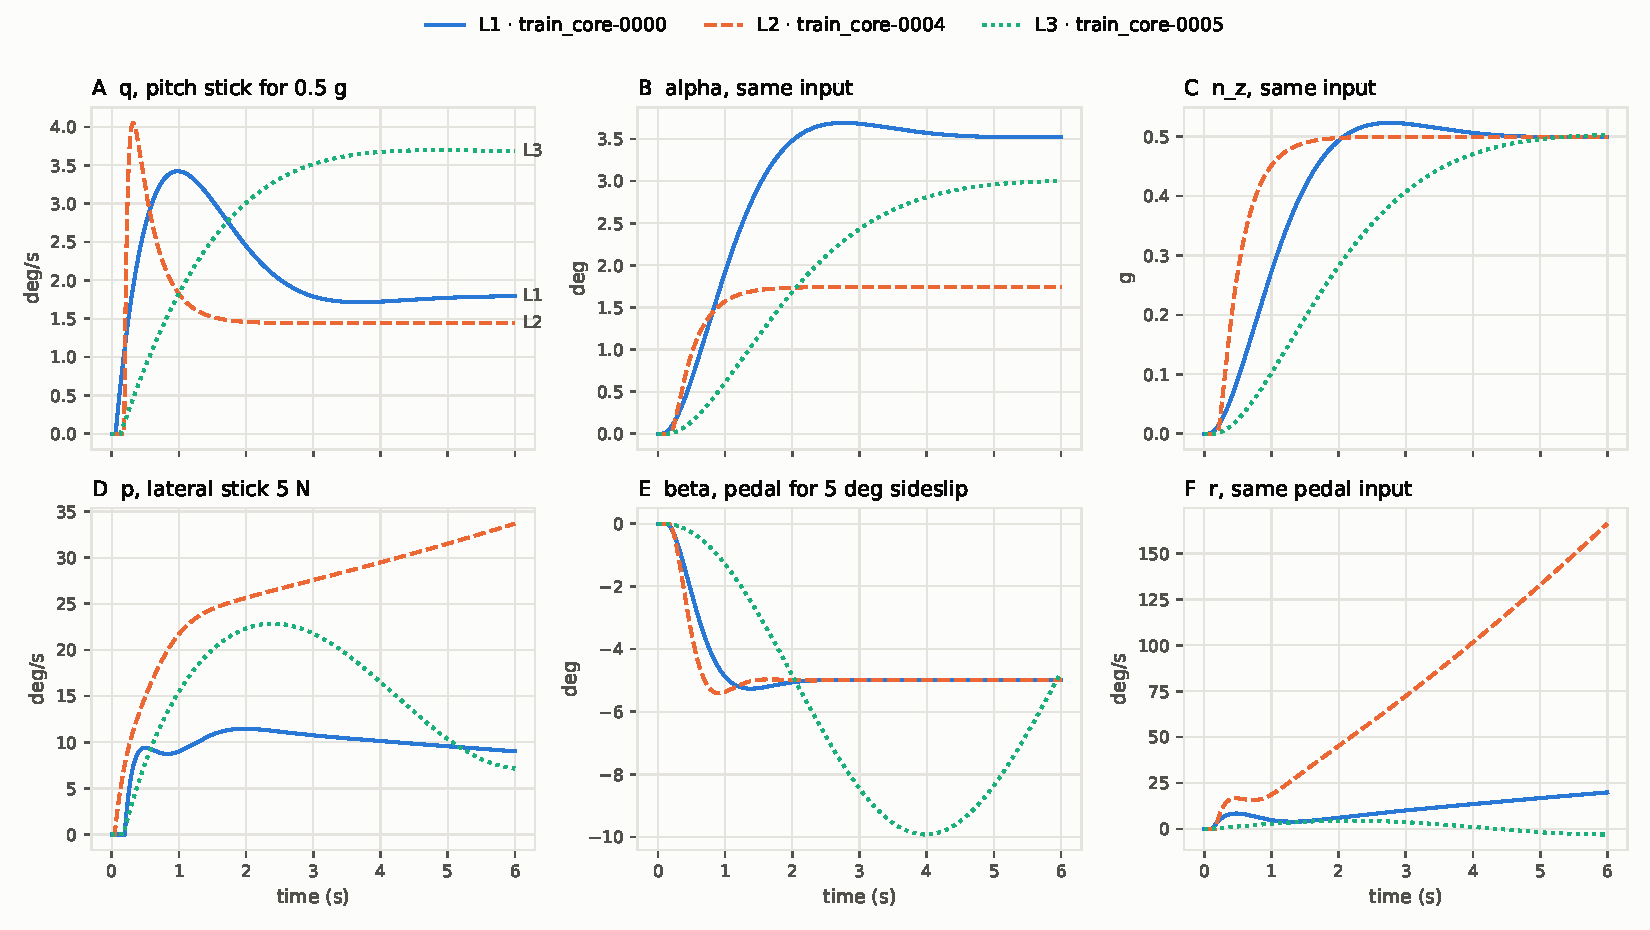
\includegraphics[width=\linewidth]{figures/step_responses.pdf}
\caption{v1 品模三个代表对象的各通道阶跃响应。A–C：俯仰杆力按 0.5 g 稳态过载给定；D：横向杆力 5 N；E–F：脚蹬力按 5° 稳态侧滑给定。2 级对象的螺旋根为正（\(\lambda_s=+0.067\)，倍幅时间不短于 8 s），开环下 \(p\) 与 \(r\) 持续增长；3 级对象的荷兰滚阻尼仅 0.005。}
\label{fig:v1}
\end{figure}

v1 的横航向通道彼此解耦：\(\beta/F_{as}\)、\(p/F_{rp}\) 等交叉通道为零，速度保持配平值，没有油门、重力耦合与湍流。第~\ref{sec:v2} 节逐项处理这些问题。

\section{交叉通道与耦合动力学}
\label{sec:v2}
\subsection{横航向四状态与保持滚转通道的反解}
表~\ref{tab:channels} 中的三条横航向通道共用同一组模态 \((T_R,\lambda_s,\zeta_d,\omega_d)\)，说明它们是同一个横航向系统的不同输出。v2 采用 Etkin、Nelson 教材的稳定轴四状态 \([\beta,p,r,\phi]\)：
\begin{equation}
\begin{aligned}
\dot\beta&=Y_\beta\beta-r+g'\phi+Y_{rp}F_{rp},\\
\dot p&=L'_\beta\beta+L'_p p+L'_r r+L_aF_{as}+L'_{rp}F_{rp},\\
\dot r&=N'_\beta\beta+N'_p p+N'_r r+N_aF_{as}+N'_{rp}F_{rp},\qquad \dot\phi=p,
\end{aligned}
\end{equation}
其中 \(g'=g/V_0\)，各输入带相应的传输延迟。同一组极点自然给出 \(p,\beta,r\) 对两路输入的全部六条通道，滚转通道为
\begin{equation}
\frac{p}{F_{as}}=\frac{L_a\,s\,\bigl[s^2+(L'_r\eta-N'_r-Y_\beta)s+N'_\beta+N'_rY_\beta-\eta(L'_\beta+L'_rY_\beta)\bigr]}{\Delta_{\mathrm{lat}}(s)}\,e^{-\tau_p s},\qquad \eta=\frac{N_a}{L_a}.
\end{equation}

现有 5,000 个对象的 \(p/F_{as}\) 是冻结的。以它为约束，特征多项式 4 个系数与分子 2 个系数构成 6 个方程，未知量为 \(Y_\beta,L'_\beta,L'_p,L'_r,N'_\beta,N'_p,N'_r\) 与副翼偏航比 \(\eta\) 共 8 个。给定 \(Y_\beta\) 与 \(L'_r\) 后，剩余方程对 \(\eta\) 是一次的，全部导数有唯一闭式解；全库复算的极点与分子系数误差约 \(10^{-13}\)。也就是说，\textbf{交叉通道大部分已由现有滚转库决定，可选的只有两维。}反解同时揭示了两条物理关系：
\begin{equation}
a_0=g'\bigl(L'_\beta N'_r-L'_rN'_\beta\bigr)=-\frac{\lambda_s\,\omega_d^2}{T_R},\qquad \frac{\omega_\phi^2}{\omega_d^2}\approx 1+\eta\,\Bigl|\frac{\phi}{\beta}\Bigr|_d .
\end{equation}
前者表明螺旋根几乎单独决定上反：螺旋稳定、滚转快的对象需要强上反，螺旋发散只说明上反相对不足。后者即 Davidson 与 Andrisani 的式 (3.22)：原库独立采样的 \(\omega_\phi/\omega_d\) 由此确定了副翼偏航。

\subsection{长周期、大机动与扰动}
纵向扩展为四状态 \([u,\alpha,q,\theta]\) 并加入油门 \(\delta_T\)（推力增量/重量，发动机按 1 s 一阶滞后）：
\begin{equation}
\begin{aligned}
\dot u&=X_uu+X_\alpha\alpha-g\theta+g\,\delta_T, &\qquad \dot\alpha&=Z_uu+Z_\alpha\alpha+q,\\
\dot q&=M_uu+M_\alpha\alpha+M_qq+K_\theta F_s(t-\tau_\theta), & \dot\theta&=q .
\end{aligned}
\end{equation}
速度导数按物理关系给定：升力正比 \(V^2\) 给出 \(Z_u=-2g/V_0^2\)，由有效升阻比给 \(X_u\)、由阻力斜率给 \(X_\alpha\)，\(M_u\) 取亚音速数据。在保持 GJB 短周期极点、零点 \(-1/T_{\theta2}\) 与 \(K_\theta\) 不变的条件下，长周期系数满足一个 \(2\times2\) 线性方程，长周期 \(\omega_p,\zeta_p\) 与 \(1/T_{\theta1}\) 作为物理结果得出；全库短周期因子保持精确（\(10^{-11}\)）。

大机动保留风轴重力分量与 \(\dot\alpha,\dot\beta\) 的运动学项（Stevens 与 Lewis 风轴力方程），配平点处它们为零，小幅响应与线性模型相差不超过 \(2\times10^{-3}\)。力矩方程使用含 \(I_{xz}\) 的完整欧拉方程：
\begin{equation}
\begin{aligned}
I_x\dot p-I_{xz}\dot r&=(I_y-I_z)qr+I_{xz}pq+\mathcal L,\\
I_y\dot q&=(I_z-I_x)pr+I_{xz}(r^2-p^2)+\mathcal M,\\
I_z\dot r-I_{xz}\dot p&=(I_x-I_y)pq-I_{xz}qr+\mathcal N .
\end{aligned}
\end{equation}
惯量比取 CR-2144 战斗机数据。湍流按 MIL-STD-1797A 4.9.2 的 Dryden 谱成形滤波器实现，中高空与低空强度、尺度按其图 262、266、267 取值，并且只经气动项进入（作用于相对气流状态 \(\mathbf x-\mathbf x_g\)）；线速度分量方差的解析值等于 \(\sigma^2\)，仿真记录相差 2–3\%。另增加理想直接法向力输入，对应思维导图的“直接法向力操纵”。

\subsection{品质判据}
v2 新增可计算的横航向判据，与滚转、俯仰判据共同构成表~\ref{tab:criteria}（IV 类、A 种阶段、中央杆）。判据先在 CR-2144 的真实飞机上运行检验：F-104A、F-4C 为 1 级，NT-33A 进场状态荷兰滚慢且阻尼小，为 3 级。

\begin{table}[H]
\centering\small
\caption{对象定级所用的品质判据（1 / 2 / 3 级）}\label{tab:criteria}
\begin{tabularx}{\linewidth}{@{}l>{\raggedright\arraybackslash}p{0.38\linewidth}Y@{}}
\toprule
判据 & 量 & 边界与出处 \\
\midrule
滚转模态 & \(T_R\) & \(\le\) 1.0 / 1.4 / 10 s；GJB 表 A18 \\
螺旋模态 & 倍幅时间 \(T_2=\ln2/\lambda_s\) & \(\ge\) 12 / 8 / 4 s；GJB 表 A19 \\
滚转灵敏度 & \(S_{1s}=|\phi(1\,\mathrm s)|/F_{as}\) & \(\le\) 3.38 / 5.62 deg/N；GJB 表 A31 \\
滚转延迟 & \(p/F_{as}\) 的等效延迟 \(\tau_p\)（v4 起） & \(\le\) 0.10 / 0.20 / 0.25 s；GJB 表 A21 \\
荷兰滚 & \(\zeta_d,\ \zeta_d\omega_d,\ \omega_d\)，含 \(\omega_d^2|\phi/\beta|_d\) 修正 & GJB 表 A35；MIL 表 XL \\
滚转振荡 & \(p_{osc}/p_{av}\)，随 \(\psi_\beta\) & MIL 4.5.1.4；\(|\phi/\beta|_d<1.5\) 不评 \\
侧滑偏离 & \(\Delta\beta/k\)，\(k\) 按速度段 & MIL 4.6.2；GJB 图 A186–A189 \\
定常侧滑方向 & 上反与脚蹬方向 & 各级都要求；MIL 4.5.5、4.6.1.2 \\
短周期频率 & \(\mathrm{CAP}=\omega_{sp}^2/(n/\alpha)\) & 0.28–3.6 且 \(\omega_{sp}\ge1\) / 0.16–10 且 \(\omega_{sp}\ge0.6\)；GJB 图 A3(a) \\
短周期阻尼 & \(\zeta_{sp}\) & 0.35–1.30 / 0.25–2.00；GJB 表 A6 \\
俯仰延迟 & \(\tau_\theta\) & \(\le\) 0.10 / 0.20 / 0.30 s；GJB 表 A7 \\
每 g 杆力 & \(F_s/n\)，\(n_L=7\) & GJB 表 A10(a) \\
长周期 & \(\zeta_p\)，\(T_2=-0.693/(\zeta_p\omega_p)\) & \(\ge0.04\) / \(\ge0\) / \(T_2\ge55\) s；GJB 表 A5 \\
长周期零点 & \(1/T_{\theta1}\)（v4 起） & 各级都要求 \(>0\)；GJB 表 A4 \\
\bottomrule
\end{tabularx}
\end{table}

\subsection{结果：滚转库在其余通道上的表现}
v2 库 \code{coupled\_six\_channel\_5000\_v2} 为 5,000 个原对象补上耦合导数、交叉轴等级与长周期，原滚转参数与 v1 字段不变。真实性检查对每个对象在 \(Y_\beta\times L'_r\) 的 \(9\times81\) 网格上反解，用 CR-2144 的 94 个真实飞行状态检查 7 个归一化量（上反比 \(-L'_\beta/N'_\beta\)、\(N'_\beta/\omega_d^2\)、\(L'_pT_R\)、\(N'_r/(2\zeta_d\omega_d)\)、\(N'_p/L'_p\)、\(L'_r/N'_r\)、\(\eta\)），接受范围取真实状态的完整范围。

\begin{table}[H]
\centering\small
\caption{v2：原滚转对象的导数能否落入真实飞机范围}\label{tab:v2real}
\begin{tabular}{@{}lrrr@{}}
\toprule
原滚转等级 & 落在真实范围内 & 其中不降级 & 只能取最近点 \\
\midrule
1 级 & 832 / 1,500（55\%） & 151 & 668 \\
2 级 & 829 / 1,500（55\%） & 341 & 671 \\
3 级 & 497 / 1,500（33\%） & 497 & 1,003 \\
OOD & 176 / 500（35\%） & 30 & 324 \\
\midrule
合计 & 2,334 / 5,000（47\%） & & \\
\bottomrule
\end{tabular}
\end{table}

表~\ref{tab:v2real} 显示，47\% 的对象能找到落在真实范围内的导数。越界最多的是 \(N'_p/L'_p\)（1,654 个）与 \(N'_\beta/\omega_d^2\)（1,163 个），原因是原库逐项独立采样极点与零点 \(\omega_\phi,\zeta_\phi\)，而真实飞机中它们由同一组导数决定。

\begin{table}[H]
\centering\small
\caption{v2：原滚转 1 级的 1,500 个对象在新增横航向判据下的等级}\label{tab:v2cross}
\begin{tabular}{@{}lrrr@{}}
\toprule
判据 & 1 级 & 2 级 & 3 级 \\
\midrule
荷兰滚（含 \(\omega_d^2|\phi/\beta|_d\) 修正） & 1,464 & 33 & 3 \\
滚转振荡 \(p_{osc}/p_{av}\) & 1,191 & 229 & 80 \\
侧滑偏离 \(\Delta\beta/k\)，中速段 & 224 & 358 & 918 \\
侧滑偏离 \(\Delta\beta/k\)，低速段 & 554 & 521 & 425 \\
以上最差（中速段） & 203 & 376 & 921 \\
\bottomrule
\end{tabular}
\end{table}

侧滑偏离是主要的降级来源（表~\ref{tab:v2cross}）。降到 3 级的对象荷兰滚频率中位数为 1.30 rad/s，1 级对象为 3.93 rad/s；去掉重力项后 3 级比例基本不变，说明降级来自对象自身的模态组合。长周期方面，667 个对象（13\%）倍幅时间短于 55 s，其中 647 个为非周期的速度/航迹发散，且与短周期过阻尼强相关：\(\zeta_{sp}\) 最高四分位（\(>1.14\)）的发散率为 39\%，最低四分位为 2\%。

把滚转原等级、纵向短周期、交叉轴（中速段）与长周期取最差项，原 1 级的 1,500 个对象中仍为 1 级的只有 141 个（9\%）。\textbf{现有 5,000 对象库作为滚转单通道库是自洽的；补齐其余通道后，大多数对象不再保持原来的等级。}原因在于 LOES 参数在各通道独立采样，而真实飞机的横航向与纵向模态由同一组导数联系。

图~\ref{fig:v2cross} 对照了耦合模型与思维导图解耦式的响应，图~\ref{fig:v2maneuver} 给出大机动与扰动下的验证。

\begin{figure}[H]
\centering
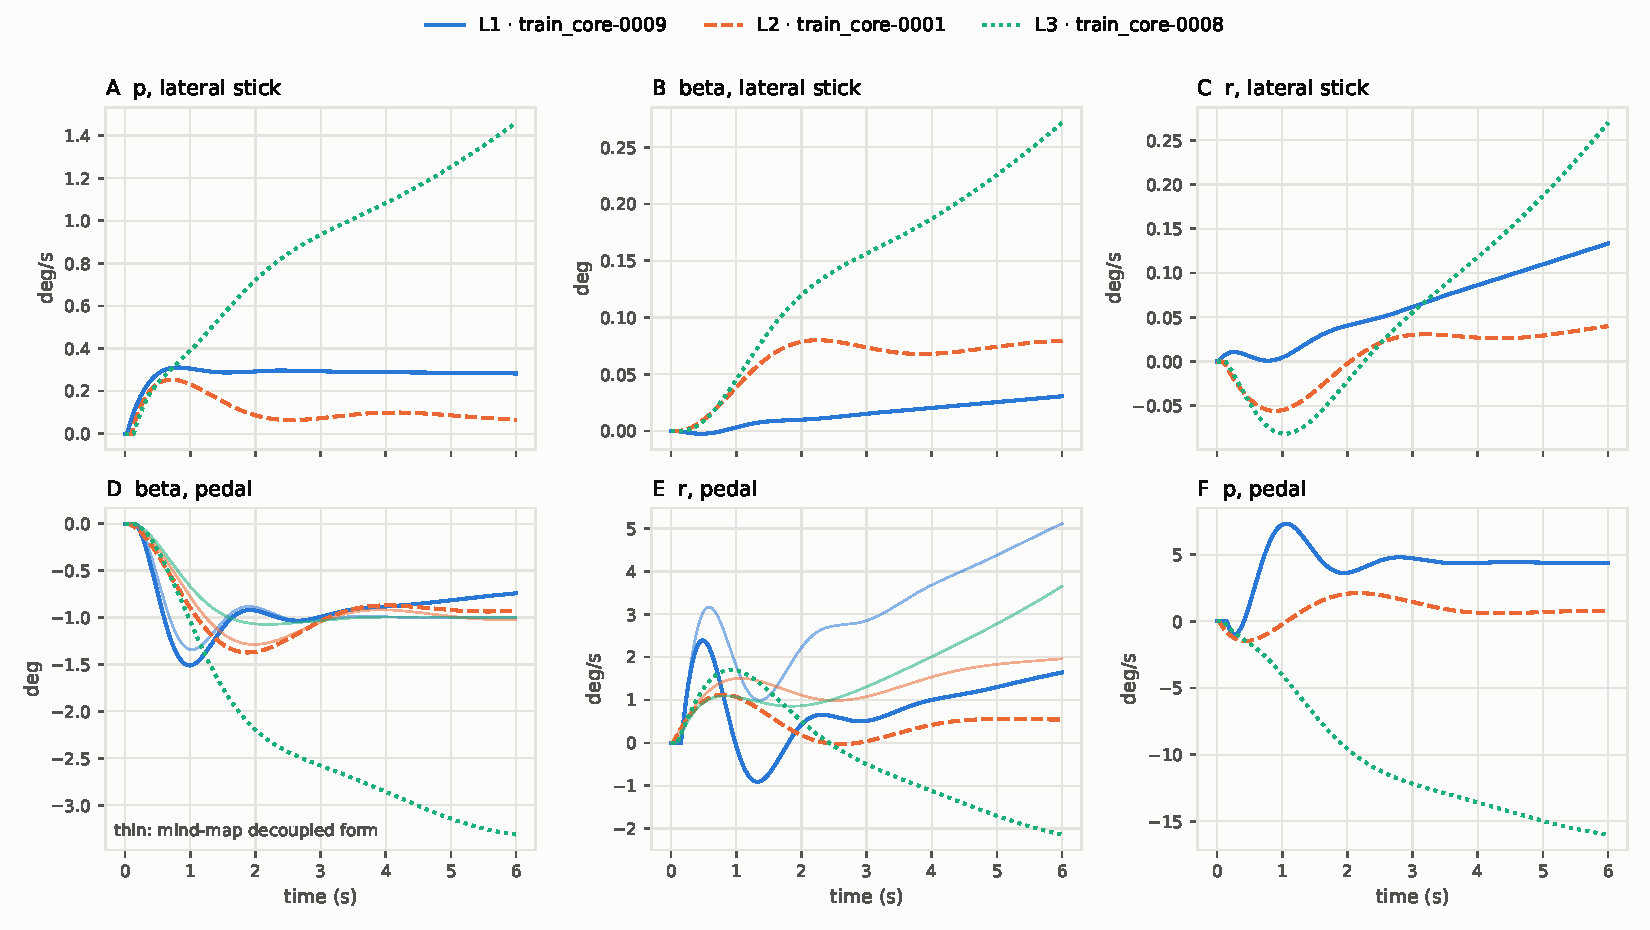
\includegraphics[width=\linewidth]{figures/cross_channels_v2.pdf}
\caption{v2 耦合模型的交叉通道响应。A–C：横向杆输入下的 \(p,\beta,r\)；D–F：脚蹬输入下的 \(\beta,r,p\)。D、E 中的细线为思维导图的解耦式，粗线为耦合模型。方向舵位于重心上方，右蹬先产生左滚力矩，随后由上反带出右滚。}
\label{fig:v2cross}
\end{figure}

\begin{figure}[H]
\centering
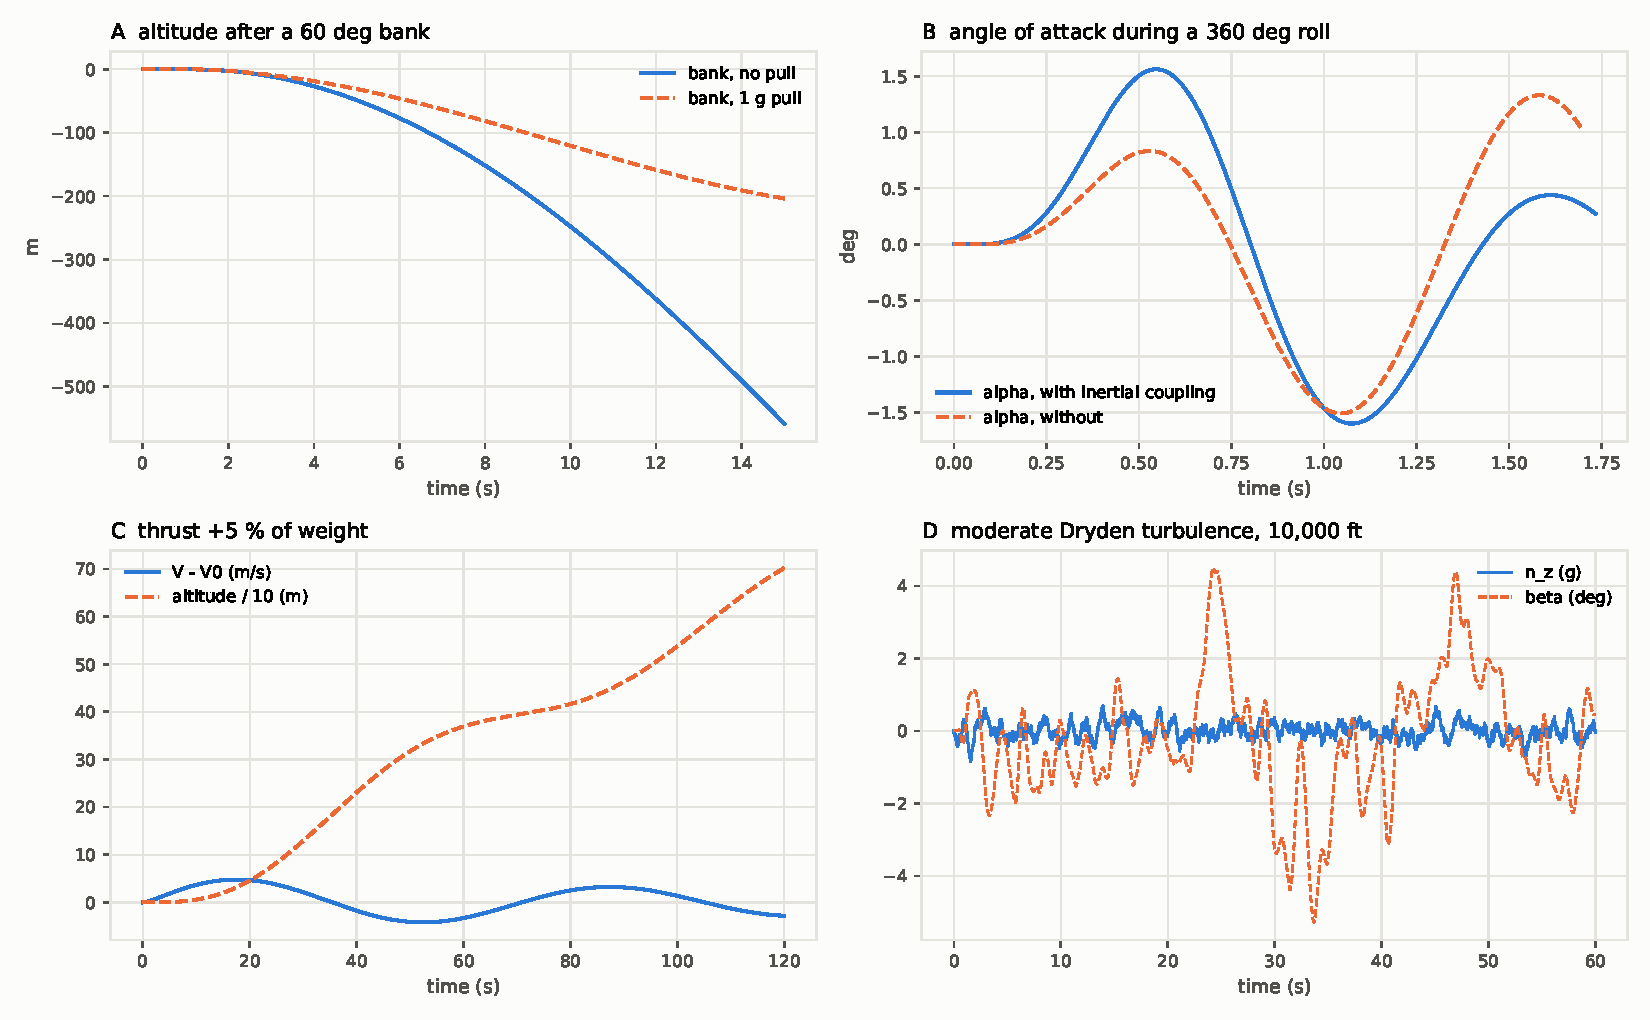
\includegraphics[width=\linewidth]{figures/large_maneuvers_v2.pdf}
\caption{v2 全量动力学的大机动与扰动验证（坐标轴转动项修正后重算）。A：压坡度 60° 不拉杆，15 s 掉高 558 m，拉 1 g 后掉高 204 m；B：约 205°/s 的 360° 滚转，有惯性耦合时迎角最大偏离 1.6°；C：推力增加 5\% 重量，120 s 内爬升约 700 m，速度按约 70 s 周期的长周期振荡；D：中高空中度 Dryden 湍流（\(\sigma=3.05\) m/s），\(n_z\) 均方根 0.23 g，\(\beta\) 均方根 1.7°。}
\label{fig:v2maneuver}
\end{figure}

\section{品质优先的重新采样（v3）}
\label{sec:v3}
v2 的结论指向重新采样：既然横航向模态、零点与交叉通道由同一组导数联系，就应在导数层面保证真实性，同时在模态层面保留“基于飞行品质的对象族”这条主线。v3 的构造分为六步。

\begin{enumerate}[leftmargin=2em]
\item \textbf{模态按 GJB 等级采样}，规则与原 IV-A 库相同：\(T_R\)、螺旋 \(\lambda_s\)、荷兰滚 \(\zeta_d/\omega_d\)、1 s 滚转灵敏度与俯仰短周期。2、3 级桶轮流把一项推到该级，其余留在 1 级。
\item \textbf{耦合形状取自 CR-2144}：\(Y_\beta\)、\(N'_p/L'_p\)、\(L'_r/N'_r\)、\(\eta\) 按 5–95 百分位抽取；方向舵滚转比与侧力比按真实分位数、并分别相对上反比与 \(Y_\beta/N'_\beta\) 抽取。两者都由垂尾决定，相对抽取使上反方向合格率由 v2 独立抽取时的 41\% 升至 82\%，接近真实飞机的 84\%。
\item \textbf{由模态与形状精确解出导数。}记 \(S=-a_3-Y_\beta\)、\(c_1=N'_p/L'_p\)、\(c_2=L'_r/N'_r\)，全部导数都是 \(L'_p\) 的函数：
\begin{equation}
N'_r=S-L'_p,\quad N'_p=c_1L'_p,\quad L'_r=c_2N'_r,\quad N'_\beta=a_2-L'_pN'_r-Y_\beta S+L'_rN'_p,
\end{equation}
\(L'_\beta\) 由 \(a_1\) 式给出，代入 \(g'(L'_\beta N'_r-L'_rN'_\beta)=a_0\) 得到关于 \(L'_p\) 的四次方程，取落在真实范围内的实根。滚转零点 \(\omega_\phi,\zeta_\phi\) 与全部交叉通道因此都是推导量。
\item \textbf{纵向}：\(\zeta_{sp}\le1.2\)、\(\omega_{sp}\le12\) rad/s（CR-2144 实测最大值分别为 0.885 与 10.2）；长周期由亚音速导数得出并参与评级。
\item \textbf{飞行包线}：每个对象带 \(V_{\min}\in[50,70]\) m/s 与 \(V_{\max}\in[260,400]\) m/s，按 GJB 速度段确定侧滑偏离中的 \(k\)。
\item \textbf{全部判据参与综合等级}，取最差项。按综合等级凑满 1/2/3 级各 1,500 个与 OOD 500 个，划分沿用原库；每级内部按定级来源轮流选取。
\end{enumerate}

65,536 个候选中 45,420 个（69\%）对应真实飞机，各级候选池均满足配额。推导出的 \(\omega_\phi/\omega_d\) 的 5–95 百分位为 0.70–1.12，与 CR-2144 的 0.64–1.13 一致，而原库在 0.65–1.35 间均匀分布。荷兰滚频率中位数由原库的 2.0 rad/s 升至 3.4 rad/s，原因是低频荷兰滚很难满足侧滑偏离判据。v3 共 35 项测试通过。

\section{合理性检查与 v4 对象库}
\label{sec:v4}
\subsection{检查方法与已修正的问题}
合理性检查用 sympy 复推公式页的全部传递函数、特征多项式系数与反解式，在 v3 的 5,000 个对象上复算极点、零点与短周期因子（误差不超过 \(4\times10^{-11}\)），与 CR-2144 真实飞机比对导数量纲，并由独立代理复核。公式推导无误，检查修正了以下问题：
\begin{itemize}[leftmargin=1.5em]
\item \textbf{稳定轴转动项。}原实现按当前迎角把稳定轴角速度换算到机体轴，漏了 \(\dot\alpha\,r_s\) 与 \(-\dot\alpha\,p_s\) 两项，无力矩翻滚 2 s 的角动量相对误差达 1.69。现按配平迎角把稳定轴固连在机体上（导数所在的轴），力方程的运动学项用当前迎角，误差降至 \(5\times10^{-3}\) 以内，并新增角动量守恒测试。小幅响应与 v3 验证数值不变，v2 大机动数值已重算（图~\ref{fig:v2maneuver}）。
\item \textbf{机动标定。}360° 滚转按对象速度段的 1 级滚转性能标定杆力，迎角变化或侧滑超过 15° 即停止并标出，同时给出 Phillips 临界滚转角速度；60° 压坡度按线性横航向模型标定脉冲。
\item \textbf{表述与标签。}更正“螺旋发散一律下反”的表述；慢滚转与稳定螺旋相近时，取最接近 \(-1/T_R\) 的实根为滚转模态。
\end{itemize}

另有七项问题需要重新采样才能修正，包括滚转等效延迟未定级、标准对各级都要求的项被计为 3 级、\(1/T_{\theta1}>0\) 未检查等。按标准同时改判后，v3 的 1/2/3 级与 OOD 由 1500/1500/1500/500 变为 742/2207/866/1185。v3 原样保留，修正在 v4 中进行。

\subsection{v4 的修正}
v4 的构造方式与 v3 相同，配额与划分不变，修正内容见表~\ref{tab:v4fix}。

\begin{table}[H]
\centering\small
\caption{v3 的问题与 v4 的处理}\label{tab:v4fix}
\begin{tabularx}{\linewidth}{@{}>{\raggedright\arraybackslash}p{0.25\linewidth}>{\raggedright\arraybackslash}p{0.36\linewidth}Y@{}}
\toprule
v3 的问题 & v4 的处理 & v4 结果 \\
\midrule
滚转等效延迟 \(\tau_p\) 未定级 & 按 GJB 表 A21 定级并按级采样 & 1 级 \(\tau_p\le0.10\) s；以延迟定级的 2 级 131 个、3 级 163 个 \\
定常侧滑方向不满足计 3 级 & 归入 OOD（标准对各级都要求） & OOD 128 个 \\
长周期实根发散按 \(T_2\) 计 3 级 & 归入 OOD（GJB 表 A5 的 3 级要求 \(|\zeta_p|<1\)） & OOD 50 个 \\
\(1/T_{\theta1}\le0\) 未检查 & 归入 OOD（GJB 表 A4） & OOD 50 个 \\
存在 \(M_q>0\)、\(N'_r>0\) & 不作为候选 & 0 个 \\
\(L'_r/N'_r\) 在 5–95 百分位内均匀抽取 & 按 94 个状态的 2.5–97.5 百分位分位数抽取 & \(L'_r\) 中位数 4.6 → 3.6，超出真实范围 33\% → 22\% \\
配平迎角固定 0.05 rad & \(\alpha_0=1/(n/\alpha)+\delta\)，\(\delta\in[-4.3^\circ,3.0^\circ]\) 取自战斗机清洁构型 & \(\alpha_0\) 中位数 4.2°，5–95 百分位 \(-1.1^\circ\)…12.6° \\
\(I_{xz}/I_x\) 独立均匀抽取 & 由惯性主轴倾角 \(\varepsilon\in[0.82^\circ,2.86^\circ]\) 给出：\(I_{xz}=\tfrac12(I_z-I_x)\tan2\varepsilon\) & \(I_{xz}/I_y\le0.05\) \\
\bottomrule
\end{tabularx}
\end{table}

\subsection{v4 的结果}
65,536 个候选中 49,539 个（75.6\%）可对应真实飞机（v3 为 45,420 个），候选池为 1 级 5,864、2 级 12,694、3 级 11,564、OOD 19,417，配额全部满足。每级按定级来源轮流选取，单项锚定的约 130 个（2 级）至 163 个（3 级）；侧滑偏离常与锚定项同时达到该级，在 2 级中涉及 788 个对象，在 3 级中涉及 545 个。OOD 的 11 类原因各约 45–90 个，定常侧滑方向为 128 个（一个对象可同时有多项原因）。速度段分布为中速 3,613、低速 859、高速 446、极低速 82。

图~\ref{fig:v4dist} 对比了 v4 与原滚转库的参数分布。\(T_R\) 中位数保持在 0.53 s；\(\zeta_d\) 的 5 百分位由原库的 0.01 升至 0.22，原库 3 级中极弱阻尼的荷兰滚对象大幅减少；\(\omega_\phi/\omega_d\) 的 5–95 百分位为 0.73–1.10，集中在真实飞机所在的 1 附近。360° 滚转按 1 级滚转性能给杆时，每 50 个对象抽 1 个，迎角偏离中位数为 3.1°（v3 为 6.6°）；有惯性耦合时 100 个抽样中有 10 个超出 15° 线性范围，无耦合时为 4 个。v4 共 45 项测试通过（v1 14 项、耦合 16 项、v3 6 项、v4 9 项），逐对象检查配额与划分、滚转通道与短周期精确、等级可由存储参数重新算出，以及能从配平点正常仿真。

\begin{figure}[H]
\centering
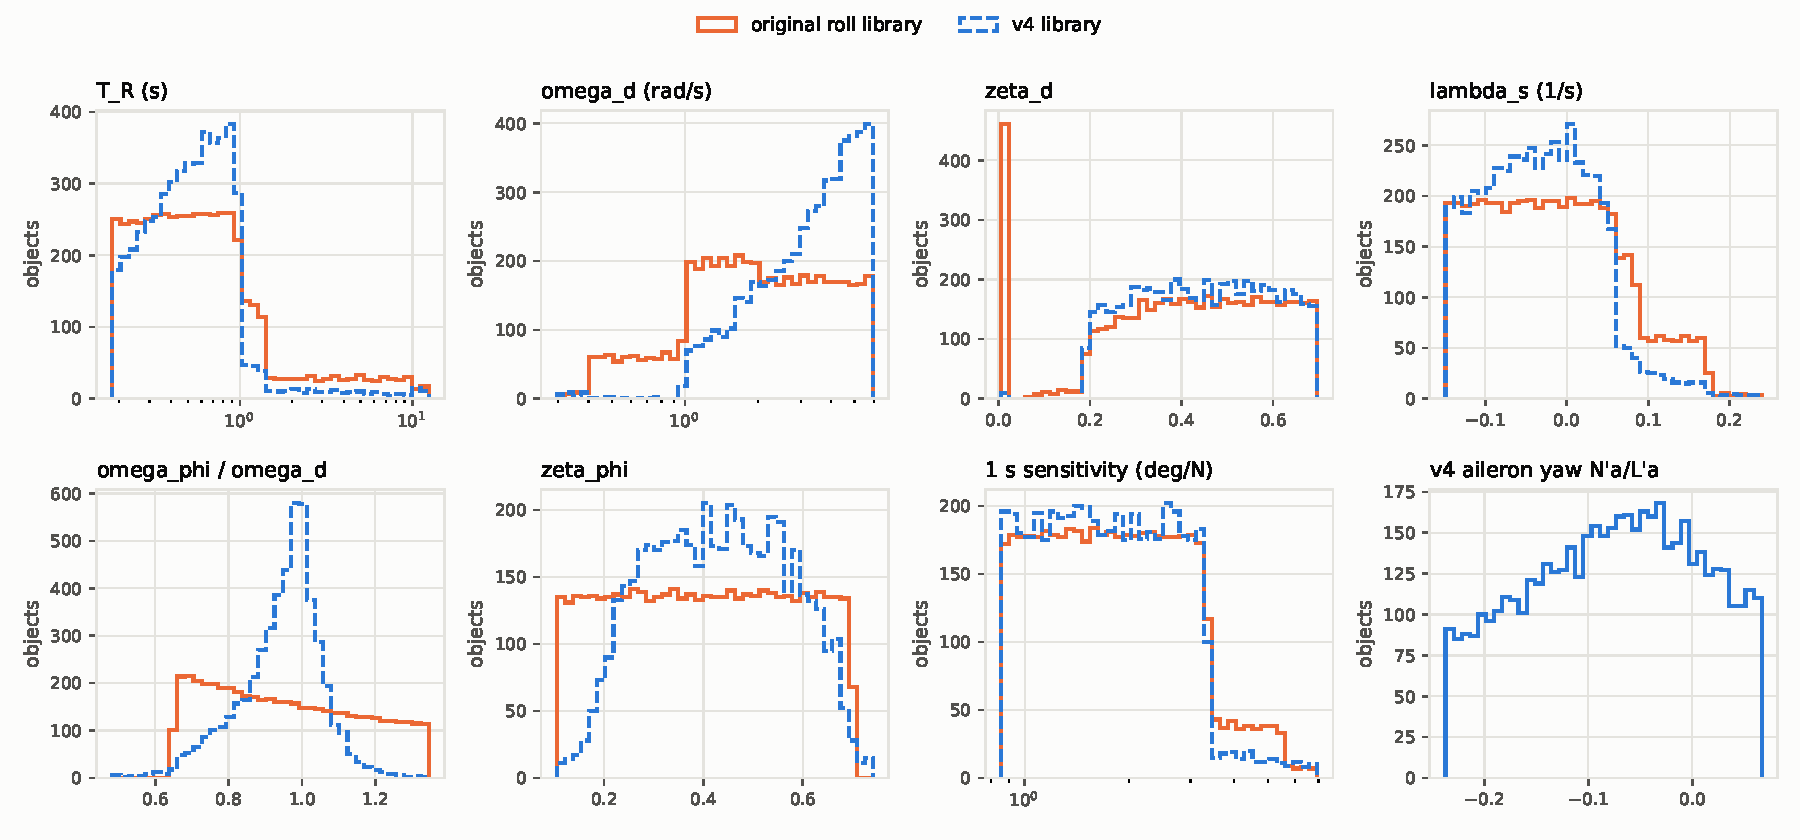
\includegraphics[width=\linewidth]{figures/distributions_v4.pdf}
\caption{v4 对象库（虚线）与原滚转库（实线）的参数分布。前七项为滚转与荷兰滚模态参数、滚转零点与 1 s 灵敏度，最后一项为 v4 推导得到的副翼偏航比 \(N'_a/L'_a\)。}
\label{fig:v4dist}
\end{figure}

\begin{figure}[H]
\centering
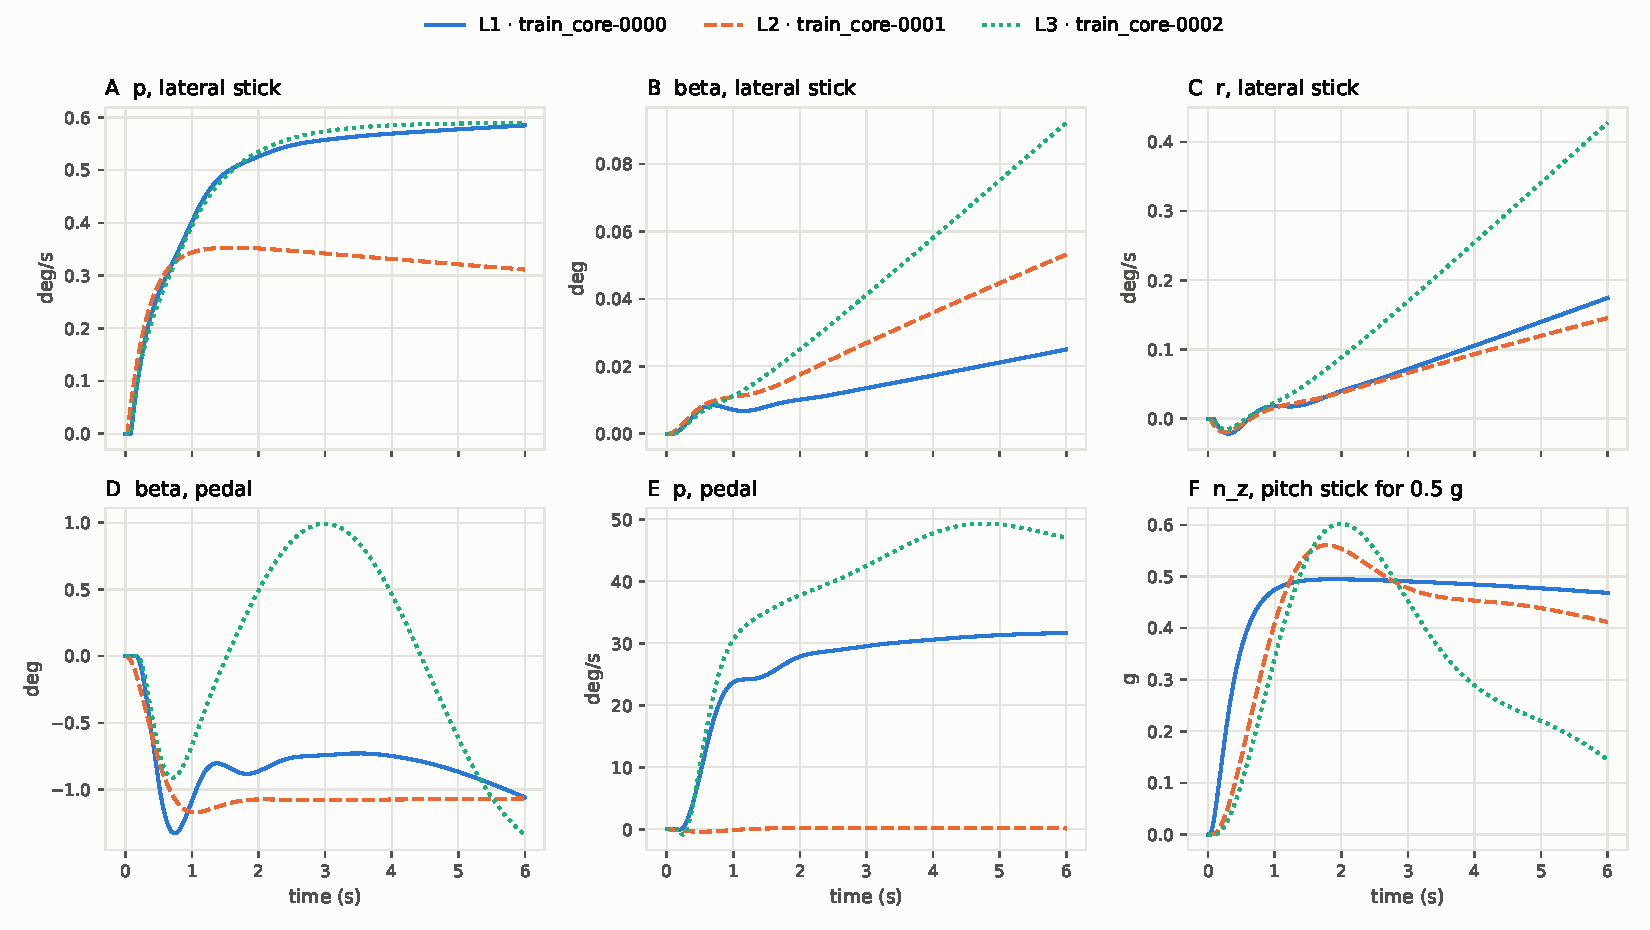
\includegraphics[width=\linewidth]{figures/responses_v4.pdf}
\caption{v4 三个代表对象的耦合响应。A–C：横向杆输入下的 \(p,\beta,r\)；D–E：脚蹬输入下的 \(\beta,p\)；F：俯仰杆力按 0.5 g 给定时的 \(n_z\)。1 级对象 train\_core-0000 位于中速段；2 级对象 train\_core-0001 与 3 级对象 train\_core-0002 均由长周期定级，后者位于极低速段。}
\label{fig:v4resp}
\end{figure}

表~\ref{tab:versions} 汇总了四个版本对象库的构造方式与主要指标。

\begin{table}[H]
\centering\small
\caption{六通道对象库各版本对照}\label{tab:versions}
\begin{tabularx}{\linewidth}{@{}l>{\raggedright\arraybackslash}p{0.35\linewidth}Yr@{}}
\toprule
版本 & 构造 & 主要结果 & 测试 \\
\midrule
v1 & 原滚转对象逐个补充纵向、脚蹬与惯性参数；通道解耦 & 配额与原库一致；六个输出与连续传递函数误差 \(<10^{-6}\) & 14 \\
v2 & 保持冻结 \(p/F_{as}\)，在 \(Y_\beta\times L'_r\) 上反解耦合导数；加长周期、惯性耦合、湍流 & 47\% 对应真实飞机；原 1 级仅 9\% 综合仍为 1 级；13\% 长周期快速发散 & 29 \\
v3 & 模态按 GJB 采样，形状取自 CR-2144，导数由四次方程解出；全部判据综合定级 & 候选 69\% 对应真实飞机；\(\omega_\phi/\omega_d\) 0.70–1.12 & 35 \\
v4 & v3 构造加滚转延迟定级、标准 OOD 归类、导数符号与真实分位数、配平迎角与主轴倾角 & 候选 75.6\% 对应真实飞机；\(\omega_\phi/\omega_d\) 0.73–1.10；1/2/3/OOD = 1500/1500/1500/500 & 45 \\
\bottomrule
\end{tabularx}
\end{table}

\section{可视化与复现}
\label{sec:web}
对象库观察服务位于 \code{six\_channel\_model\_2026-10-29/web}，以 \code{python start.py} 启动，监听 127.0.0.1:8330，只读访问对象库，当前版本为 \code{six-channel-v4-viewer-2026-10-31}。主页“模型与公式”用本地 KaTeX 渲染从六个通道到动力学、运动学的全部推导，并对选中对象逐节代入数值，给出状态矩阵、零极点与频率响应。\code{/library} 页面给出链路说明、各级定级来源、与原滚转库及 CR-2144 真实飞机的参数分布对比、5,000 个对象的散点浏览器，以及选中对象的现场仿真（小幅阶跃与大机动）。

各版本对象库均由固定种子生成，目录已存在时拒绝覆盖。复现命令如下：
\begin{verbatim}
cd six_channel_model_2026-10-29
PYTHONDONTWRITEBYTECODE=1 python -m unittest discover -s tests   # 45 项
PYTHONDONTWRITEBYTECODE=1 python verify_v4.py
cd ../ppo_fixes_2026-10-26
PYTHONDONTWRITEBYTECODE=1 python -m unittest discover -s tests   # 8 项
\end{verbatim}

\section{后续工作}
\label{sec:next}
v4 对象库的导数是增稳后飞机的等效导数，\(N'_r\) 中位数为 \(-2.59\)，约为真实裸机（\(-0.24\)）的 10 倍；真实性约束作用在 7 个归一化比值上。尚未检查的判据包括正上反所需杆力上限、滚转性能、驾驶员位置侧向加速度与 \(\omega_{sp}T_{\theta2}\) 替代判据；大机动使用线性气动，不含失速。新对象与已训练的滚转教师不一一对应，滚转研究作为路线可行性验证保持不变。

下一步是在 v4 库上建立俯仰、滚转、脚蹬三回路的批量 GPU 环境，设计指令与奖励，先在 GPU 4 上试训单个对象，再确定教师规模。该阶段需经确认后开始。表~\ref{tab:size} 按现有网络代码给出统一学生的参数量估算：每回路沿用滚转回路的信号，另加 \(\alpha\)、\(n_z\)、\(\phi\)、\(\theta\) 四个共享量，观测由 176 维增至 660 维。

\begin{table}[H]
\centering\small
\caption{三回路统一学生的参数量估算}\label{tab:size}
\begin{tabular}{@{}lr@{}}
\toprule
统一学生结构 & 参数量 \\
\midrule
tiny 同构（卷积 8，\(32\times1\)） & 5,408 \\
加宽（卷积 16，\(64\times2\)） & 25,152 \\
small 同构（卷积 24，\(256\times4\)） & 560,416 \\
教师同构（卷积 24，\(512\times8\)） & 4,269,856 \\
\bottomrule
\end{tabular}
\end{table}

教师按每对象每回路一个，Actor 仍为 4,255,537 个参数。以 GPU 4 上滚转教师实测的每教师 142.8 卡秒外推，3,000 个对象需 9,000 个教师，约 357 卡时（五卡约 71 小时）；5,000 个对象约 595 卡时（五卡约 119 小时）。这是基于滚转教师的外推，三回路教师的实际训练难度与耗时有待实测。

\begin{thebibliography}{9}
\small
\bibitem{gjb} GJB 2874—1997. 电传操纵系统飞机的飞行品质[S]. 1997.
\bibitem{mil} MIL-STD-1797A (Notice 3). Flying Qualities of Piloted Aircraft[S]. U.S. Department of Defense, 2004.
\bibitem{cr2144} Heffley R K, Jewell W F. Aircraft Handling Qualities Data[R]. NASA CR-2144, 1972.
\bibitem{davidson} Davidson J B, Andrisani D. Lateral-Directional Eigenvector Flying Qualities Guidelines for High Performance Aircraft[R]. NASA TM-110306, 1996.
\bibitem{etkin} Etkin B, Reid L D. Dynamics of Flight: Stability and Control[M]. 3rd ed. Wiley, 1996.
\bibitem{nelson} Nelson R C. Flight Stability and Automatic Control[M]. 2nd ed. McGraw-Hill, 1998.
\bibitem{stevens} Stevens B L, Lewis F L, Johnson E N. Aircraft Control and Simulation[M]. 3rd ed. Wiley, 2016.
\bibitem{ppo} Schulman J, Wolski F, Dhariwal P, et al. Proximal Policy Optimization Algorithms[J]. arXiv:1707.06347, 2017.
\end{thebibliography}
\end{document}
